\let\negmedspace\undefined
\let\negthickspace\undefined
\documentclass[journal]{IEEEtran}
\usepackage[a5paper, margin=10mm, onecolumn]{geometry}
%\usepackage{lmodern} % Ensure lmodern is loaded for pdflatex
\usepackage{tfrupee} % Include tfrupee package

\setlength{\headheight}{1cm} % Set the height of the header box
\setlength{\headsep}{0mm}     % Set the distance between the header box and the top of the text

\usepackage{gvv-book}
\usepackage{gvv}
\usepackage{cite}
\usepackage{amsmath,amssymb,amsfonts,amsthm}
\usepackage{algorithmic}
\usepackage{graphicx}
\usepackage{textcomp}
\usepackage{xcolor}
\usepackage{txfonts}
\usepackage{listings}
\usepackage{enumitem}
\usepackage{mathtools}
\usepackage{gensymb}
\usepackage{comment}
\usepackage[breaklinks=true]{hyperref}
\usepackage{tkz-euclide} 
\usepackage{listings}
% \usepackage{gvv}                                        
\def\inputGnumericTable{}                                 
\usepackage[latin1]{inputenc}                                
\usepackage{color}                                            
\usepackage{array}                                            
\usepackage{longtable}                                       
\usepackage{calc}                                             
\usepackage{multirow}                                         
\usepackage{hhline}                                           
\usepackage{ifthen}                                           
\usepackage{lscape}
\begin{document}

\bibliographystyle{IEEEtran}
\vspace{3cm}

\title{1.6.23}
\author{EE24BTECH11001 - Aditya Tripathy
}
 \maketitle
% \newpage
% \bigskip
{\let\newpage\relax\maketitle}

\renewcommand{\thefigure}{\theenumi}
\renewcommand{\thetable}{\theenumi}
\setlength{\intextsep}{10pt} % Space between text and floats


\numberwithin{equation}{enumi}
\numberwithin{figure}{enumi}
\renewcommand{\thetable}{\theenumi}


\textbf{Question}:\\
Are $\vec{A}\brak{3, 1}, \vec{B}\brak{6, 4}$ and $\vec{C}\brak{8, 6}$ collinear?
\\
\textbf{Solution: }\\
From \brak{1.1.9.1}, Points A, B, C are defined to be collinear if
\begin{align}
	rank\myvec{\vec{B}-\vec{A} & \vec{C}-\vec{A}} = 1\\
\end{align}
So, forming the collinearity matrix and doing row operations,
\begin{align}
	\myvec{3&3\\5&5} \xrightarrow{R_2 = 3R_2-5R_1}  \myvec{3&3\\0&0}\\
\end{align}
Since there is only 1 non-zero row, rank = 1. Hence the points $\vec{A}, \vec{B}$ and $\vec{C}$ are collinear.
\begin{figure}[h!]
   \centering
   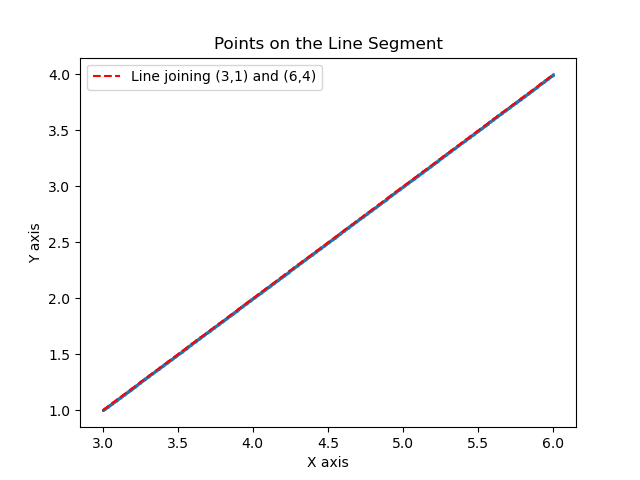
\includegraphics[width=0.7\linewidth]{figs/fig.png}
   \caption{Line joining $\vec{A}, \vec{B}$ and $\vec{C}$}
\end{figure}
\end{document}  
\end{document}
